\documentclass[a4paper]{article}
\usepackage{titling}
\usepackage{authblk}
\usepackage{fancyhdr}
\usepackage{hyperref}
\usepackage{rsc}
\usepackage{siunitx}
\usepackage{graphicx}
\usepackage{listings}
\usepackage{color}

\definecolor{dkgreen}{rgb}{0,0.6,0}
\definecolor{gray}{rgb}{0.5,0.5,0.5}
\definecolor{mauve}{rgb}{0.58,0,0.82}

\lstset{frame=tb,
  language=Python,
  aboveskip=3mm,
  belowskip=3mm,
  showstringspaces=false,
  columns=flexible,
  basicstyle={\ttfamily},
  numbers=none,
  numberstyle=\tiny\color{gray},
  keywordstyle=\color{blue},
  commentstyle=\color{dkgreen},
  stringstyle=\color{mauve},
  breaklines=true,
  breakatwhitespace=true,
  tabsize=3
}
\DeclareSIUnit\Fahrenheit{\degree F}

\title{Lecture 2: Loops, lists, arrays, optimisation, and plotting}
\author[1]{Dr Benjamin J. Morgan}
\author[1,2]{Dr Andrew R. McCluskey}
\affil[1]{Department of Chemistry, University of Bath, email: b.j.morgan@bath.ac.uk}
\affil[2]{Diamond Light Source, email: andrew.mccluskey@diamond.ac.uk}
\setcounter{Maxaffil}{0}
\renewcommand\Affilfont{\itshape\small}

\pagestyle{fancy}
\fancyhf{}
\rhead{CH40208}
\lhead{\thetitle}
\rfoot{\thepage}

\begin{document}
\maketitle

\section*{Aim}
In this lecture, you will learn about lists of objects, how to loop through them, working with arrays of numbers and how to present your findings.

\section{Lists}
The Python programming language natively includes the ability to group together a series of objects.
These are \texttt{lists} and are one of the most powerful Python objects.
Lists are an ordered set of objects, from which it is possible to pick all, one, or many values.
A list is defined as follows,
\begin{lstlisting}
# Making a list

elements = ["Hydrogen", "Helium", "Lithium", "Beryllium", "Boron", "Carbon", "Nitrogen", "Oxygen"]
\end{lstlisting}
Having defined the list, it is then possible to select individual items of the list by using the following syntax,
\begin{lstlisting}
# Printing some items

print(elements[0], elements[4], elements[-1])
\end{lstlisting}
Note, that Python starts counting from the number $0$, and using the minus sign we can ask Python to count from the end.
This means that the above code should print, \texttt{"Hydrogen", "Boron", "Oxygen"}.
This counting from $0$ means that in the above list, the string \texttt{"Hydrogen"} would be referred to as the zeroth object in the list, while \texttt{"Helium"} would be the first.

In addition to making use of single objects from within a list, it is also possible to create sublists, for example,
\begin{lstlisting}
# Just the first 4 elements

print(elements[0:4])
\end{lstlisting}
Note that above, the numbers on either side of the colon the list indices.
However, rather strangely, the sublist created is \textbf{inclusive} of the first number and \textbf{exclusive} of the second.
Additionally, it is possible to select non-consecutive objects from a list by placing commas between the indices,
\begin{lstlisting}
# Just the gases

print(elements[0, 1, 6, 7])
\end{lstlisting}
It is possible add object to the end of a list using the \texttt{append} operation,
\begin{lstlisting}
# Add more to the list

elements.append("Fluorine")
elements.append("Neon")
print(elements)
\end{lstlisting}
Additionally, items from a list can be deleted,
\begin{lstlisting}
# Deleting from a list

del elements[9]
print(elements)
\end{lstlisting}
If two lists need to be combined, this can be achieved by \emph{concatenation},
\begin{lstlisting}
# Concatenating lists
list1 = [1, 4, 6, 2]
list2 = [3, 5, 2]

print(list1 + list2)
\end{lstlisting}
More operations that may be performed on operations can be found online \url{https://docs.python.org/3/tutorial/datastructures.html}.
The final point about \texttt{lists} is that the data that they hold does not all need to be the same type.
For example, the list below contains a \texttt{float}, two \texttt{str}, a \texttt{complex} number and an \texttt{int},
\begin{lstlisting}
# List of many types

a_new_list = ['hello', 12.41242, 5 + 8j, 'sadness', 2]
print(a_new_list)
\end{lstlisting}
\vspace{\baselineskip}
\begin{center}
	\noindent\fbox{%
		\begin{minipage}{0.9\textwidth}%
			\vspace{0.15\baselineskip}
			\subsubsection*{Exercise}
			\begin{itemize}
				\item{Create two lists, one containing names the first 8 elements in the periodic table and another containing the massive numbers for those elements. Then, using a loop, print each element name and mass number, format each print statment with the \texttt{.format()} syntax.}
			\end{itemize}
		\end{minipage}
	}
\end{center}

\section{Loops}

One of the best uses of programming (and computers) is to perform repetitive task over and over.
For this we use \emph{loops}, within Python there are two common types of loop:
\begin{itemize}
	\item{\texttt{for} loops iterate over a given sequence.}
	\item{\texttt{while} loops repeat as long as a certain logical operation is \texttt{True}.}
\end{itemize}
An example of each of a \texttt{for} and \texttt{while} loop is shown below, both perform the same function,
\begin{lstlisting}
# For loop

for i in range(5):
	print(i)

i = 0
while i < 5:
	print(i)
	i = i + 1
\end{lstlisting}
Both of these code blocks will print the numbers $0$ to $4$, however the \texttt{for} loop is clearly more concise.
Additionally, the \texttt{while} loop is more prone to accidently running an \emph{infinite}.
If you were to forget to manually iterate the variable \texttt{i} (this is the line \texttt{i = i + 1}), then the \texttt{while} condition would always be \texttt{True} and therefore the code would run forever within this loop.
For this reason it is suggested that, where possible, you use a \texttt{for} loop over a \texttt{while} loop.

The \texttt{for} loop will iterate the variable (in the example above, this variable is named \texttt{i}) through whatever sequence is given (this is \texttt{range(5)} above, which is equivalent to the \emph{list} \texttt{[0, 1, 2, 3, 4]}).
The sequence does not necessarily have to be a \texttt{range} command, it may be any \texttt{list} or \texttt{numpy.ndarray} (we discuss this below).
For example, in the code below we iterate though the first ten chemical element symbols,
\begin{lstlisting}
# Printing the periodic table

elements = ["H", "He", "Li", "Be", "B", "C", "N", "O", "F", "Ne"]

for symbol in elements:
	print(symbol)

for i, symbol in enumerate(elements):
	print("The index of the list for {} is {}.".format(symbol, i)).
\end{lstlisting}
It is possible to use the \texttt{enumerate} command to count through the list during the loop, as shown in the second example above.
\vspace{\baselineskip}
\begin{center}
	\noindent\fbox{%
		\begin{minipage}{0.9\textwidth}%
			\vspace{0.15\baselineskip}
			\subsubsection*{Exercise}
			\begin{itemize}
				\item{Recall from first and second year, that Python counts indices in a list from 0. How could the above code be adapted such that the correct atomic number will be printed?}
			\end{itemize}
		\end{minipage}
	}
\end{center}

\subsection{Escaping loops}

Sometimes it is computationally efficient to leave a \texttt{for} loop, to skip a particular value, under a certain condition.
For this, the commands \texttt{break} and \texttt{continue} are available.
The \texttt{break} command will exit the \emph{inner-most} loop that is being carried out, while the \texttt{continue} command will skip the current value and jump immediately to the next.
Examples of how these may be used are shown below, where the \texttt{len} function will return the \emph{length} of the list,
\begin{lstlisting}
# Finding the zero in a list

numbers = [1, 5, 7, 0, 2, 6, 2]
for i in range(len(numbers)):
	if numbers[i] == 0:
		break

print("The zero is at index {}.".format(i))

# Making all the negative values positive

numbers = [-2, 4, 1, -5, 2, 6, -3, -4]
for i in range(len(numbers)):
	if numbers[i] >= 0:
		continue
	else:
		numbers[i] = numbers[i] * -1
\end{lstlisting}
Note that the above examples are toy problems and there are more efficient way to carry-out these specific operations in Python.

\section{NumPy Arrays}

NumPy (or \texttt{numpy} or more commonly \texttt{np}) is a library that Python can use that is designed and optimised for doing numerical operations.\cite{numpy}
Over this course you will be introduced to many other Python libraries, in order to use any of these you must \texttt{import} them,
\begin{lstlisting}
# Import NumPy

import numpy as np
\end{lstlisting}
This asks the Python interperator to go and find the NumPy library, then in order to reduce the amount of typing (programmers are lazy), we give the library the alias \texttt{np}.

One of the most powerful features of the NumPy library is the \texttt{array}, these are similar to lists but with some important differences.
Unlike a list, all of the items in a NumPy array must be of the same type; namely a NumPy data type (a list of these can be found online: \url{https://docs.scipy.org/doc/numpy/user/basics.types.html}) which are numerical data types such as \texttt{int}, \texttt{float}, and \texttt{complex}.

The power of a NumPy array comes in the ability to perform mathematical operations incredibly efficiently.
For example,\footnote{When running on a MacBook Air 2018 with a 1.6 GHz Intel Core i5.} the summation of zero to ten million is $\sim 25$ times faster when using the NumPy array operation shown below when compared with a simple implementation in pure Python,
\begin{lstlisting}
# The pure Python way

numbers = range(10000000)
total = 0
for i in numbers:
    total = total + i
print(total)

# The NumPy operation

import numpy as np

numbers = np.arange(10000000)
total = np.sum(numbers)
print(total)
\end{lstlisting}
Note that in the above example, the \texttt{range} function creates a list of numbers from $0$ to $10000000$, while the \texttt{np.arange} function creates a NumPy array containing the same values.

NumPy arrays also have a \emph{huge} amount of additional functionality, such as the ability to easily access statistically relevant values, powerful sub-array definition (in particular for multi-dimensional arrays), data reorganisation.
Some of these tools are shown below, and no doubt you will become familiar with many others throughout this course,
\begin{lstlisting}
# Determine the mean and standard deviation
import numpy as np

## First get an array of 6 numbers
x1 = np.array([2, 5, 3, 7, 2, 7])

print(x1.mean(), x1.std())

## Now get a two-dimensional array of random ints from 0 to 10
x2 = np.random.randint(10, size=(3, 2))

print(x2.shape)
print(x2)
print(x2[0])
print(x2[:, 1])
print(x2[:, 0::-1])

## Lets reshape a one-dimensional array
x3 = np.arange(10)

print(x3)
print(x3.reshape((3, 3))
\end{lstlisting}

Like other numerical types in Python, it is possible to perform mathematical operations on them (\texttt{+}, \texttt{-}, \texttt{*}, \texttt{/}, etc.).
Furthermore, additional operations are available from the NumPy library, such as statistical methods like \texttt{np.mean()}, \texttt{np.std()} (standard deviation),
\begin{lstlisting}
# Some statistical stuff!

a = np.array([1, 4, 2, 5, 3, 14])
b = np.mean(a)
c = np.std(a)
d = np.sqrt(np.sum(np.square(a-b))/a.size)
print(a, b, c, d)
\end{lstlisting}

\subsection{Optimisation with NumPy}

It was shown above, that by replacing a Pythonic loop with a NumPy array operation it was possible to get a massive speed up in computational efficiency.
This is a powerful tool of the NumPy library, that \textbf{must} be harnessed, where possible.
The general advice is that when a loop is present in code, you should consider if it would be possible to replace this with an appropriate NumPy operation.
Throughout the remainder of this module, we will make use of NumPy array operations over looping through lists whereever possible.
\vspace{\baselineskip}
\begin{center}
	\noindent\fbox{%
		\begin{minipage}{0.9\textwidth}%
			\vspace{0.15\baselineskip}
			\subsubsection*{Exercise}
			\begin{itemize}
				\item{Write some pure Python code that will calculate the average vibrational energy, $\bar{E_v}$, from the first N energy levels, $E_l$, of some diatomic molecule when,
        \begin{equation}
          \bar{E_v} = \frac{\sum_{l=0}^N{E_l p_l}}{\sum_{l=0}^N{p_l}}.
        \end{equation}
        Where, $N = 6$, the energy at each level is: 0, 1, 2, 3, 4, 5, 6 and the levels have populations, $p$: 4, 3, 2, 1, 0, 0 respectively.

        Then write a \emph{NumPy optimised} version of this code would work.}
			\end{itemize}
		\end{minipage}
	}
\end{center}

\section{Copying lists/arrays}

An important fact to be aware of for both lists and NumPy arrays is that assigning a list to an new variable does \textbf{not} create a new list.
Rather, this will create an alias to the same object in memory.
In order to create a new list (or array), it is best to \texttt{copy} the original object to the new variable, as shown below,
\begin{lstlisting}
# Copying lists and arrays

my_list = ['dog', 'cat', 'horse']

new_list = my_list

new_list[0] = 'giraffe'

print(new_list)
print(my_list)

copied_list = my_list.copy()

copied_list[1] = 'pig'

print(copied_list)
print(my_list)
\end{lstlisting}
Note that for a NumPy array, the function \texttt{np.copy(my\_array)} should be used.

\section{Plotting}

Another extremely important library that is available to the Python language is \texttt{matplotlib}, which allows plotting of data.
The \texttt{matplotlib} library was initially designed to help users of Matlab to convert there code to Python.
The use of \texttt{matplotlib} is straightforward, first you build a figure, and then add data and other items to the axes of the figure.
For example, consider the plotting of the NumPy array below,
\begin{lstlisting}
# Plotting some data
import numpy as np
import matplotlib.pyplot as plt

x = np.linspace(0, 10)
y = x ** 2

plt.plot(x, y)
plt.show()
\end{lstlisting}
This should result in a plot like that shown in Figure~\ref{fig:x2}.
%
\begin{figure}[t]
\centering
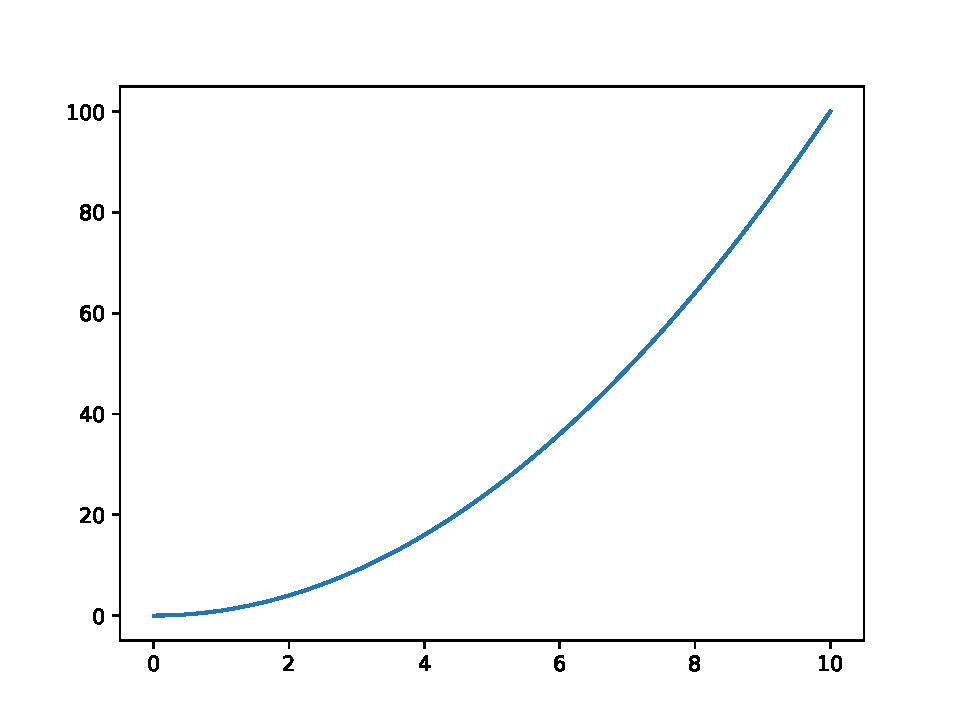
\includegraphics[width=0.8\textwidth]{x_squared}
\caption{\label{fig:x2} The result of the simple plotting script of $y = x ^ 2$.}
\end{figure}
%

The example above is rather simplistic, but the \texttt{matplotlib} library can be used to make very complex plots.
Furthermore, the example below would not to well for experimental data, considering that the axes have no labels, the data is described with a line instead of points and there is no plot title.
However, the code below shows some realistic experimental data plotted using matplotlib in a fashion that is more comprehensible.
The plot produced can be found in Figure~\ref{fig:real},
\begin{lstlisting}
# Plotting some real data
import numpy as np
import matplotlib.pyplot as plt

temperature = np.linspace(283, 363, 10)
rate_constants = np.array([3.2e-19, 3.4e-18, 3.2e-17, 2.6e-16, 1.8e-15, 1.2e-14, 7.3e-14, 3.9e-13, 1.9e-12, 8.9e-12])
rate_constants_uncertainty = np.array([1.6e-20, 1.7e-19, 1.6e-18, 1.3e-17, 9.4e-17, 6.2e-16, 3.7e-15, 2.0e-14, 1.0e-13, 4.4e-13])

plt.errorbar(temperature, rate_constants*10**12, rate_constants_uncertainty*10**12, marker='o', linestyle='')
plt.ylabel(r'Rate constant/$\times10^{-12}$ s$^{-1}$')
plt.xlabel(r'Temperature/K')
plt.title(r'Effect of temperature of rate constant of HI decomposition')
plt.tight_layout()
plt.show()
\end{lstlisting}
%
\begin{figure}[t]
\centering
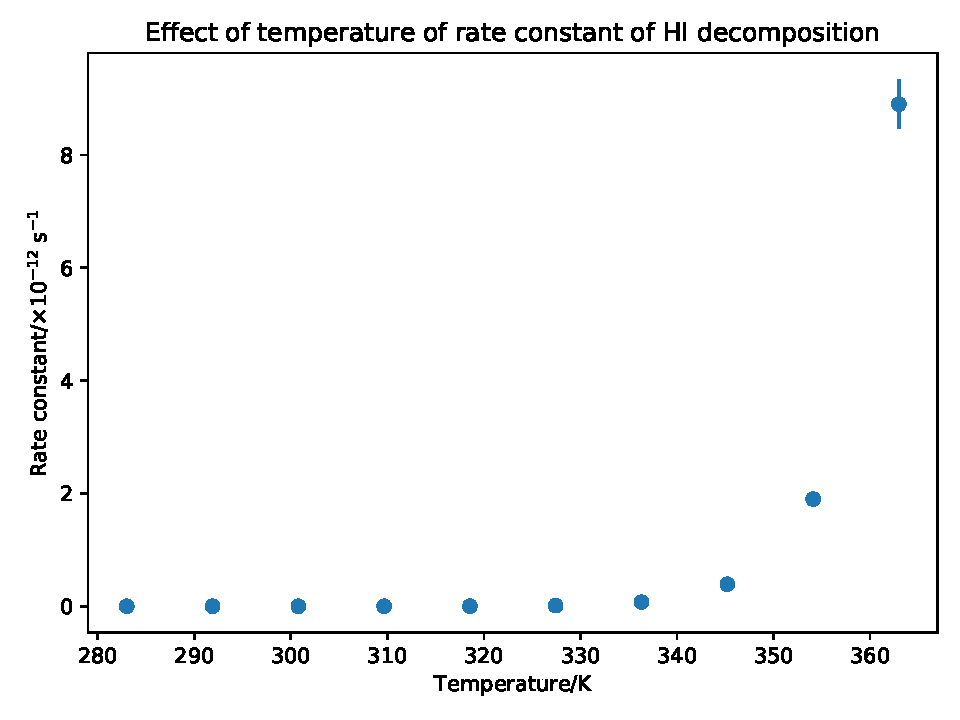
\includegraphics[width=0.8\textwidth]{real}
\caption{\label{fig:real} The result of the simple plotting script of $y = x ^ 2$.}
\end{figure}
%
\vspace{\baselineskip}
\begin{center}
	\noindent\fbox{%
		\begin{minipage}{0.9\textwidth}%
			\vspace{0.15\baselineskip}
			\subsubsection*{Exercise}
			\begin{itemize}
				\item{Read through the code used to plot the more ``realistic'' plot and determine what each element in the code does. Annotate this worksheet and ask a demonstrator to check you have all of the elements.}
			\end{itemize}
		\end{minipage}
	}
\end{center}

\section{Reading in data}

A lot of computational work in science involves processing data that has already been generated, either from a previous calculation or from an experiment. Entering data by hand (e.g.\ using \texttt{input()} is tedious, time-consuming, and error-prone.) If the data is already stored in a file, we would like to read this file directly.

The NumPy library includes the \texttt{loadtxt()} function, which will read a file containing columns of numbers and store the values as a NumPy array, making it easy to then do any subsequent analysis.
The \texttt{loadtxt()} function can take a number of additional arguments to help with parsing files formatted in specific ways\footnote{The \texttt{loadtxt()} documentation can be found at \url{https://docs.scipy.org/doc/numpy/reference/generated/numpy.loadtxt.html}.}.

The simplest example is if we have a file (called \texttt{myfile.txt}) that contains two rows of numbers separated by spaces. This can be read in using
\begin{lstlisting}
# Reading in some text

a = np.loadtxt('myfile.txt')
\end{lstlisting}
This creates a $(2\times N)$ two-dimensional NumPy array \texttt{a} (similar to a nested list). \texttt{a[0]} contains the first row of values from the file, and \texttt{a[1]} contains the second row of values.

Experimental datasets are often stored as \emph{columns} of data, instead of rows. A common filetype that uses column-formatting is the \texttt{.csv} ``comma-separated values'' format\footnote{The \texttt{.csv} format is popular for storing experimental data because it can be read directly into Microsoft Excel.}. The ``standard`` format for a \texttt{.csv} file is for the columns of data to be separated by commas (hence the name), but any characters can be used to separate, or \emph{delimit}, the columns, including whitespace (tabs or spaces)..

Reading a \text{.csv} using \texttt{loadtxt()} requires us to supply some additional arguments:
\begin{lstlisting}
# Reading in a csv file

a = np.loadtxt('myfile.csv', delimiter=',', unpack=True)
\end{lstlisting}
In this example, we pass two extra optional arguments to the function, \texttt{delimiter} defines the character that separates the values in the columns, and \texttt{unpack} indicates that the data is stored in columns rather than rows.

Data files often include comments, used to explain how and when the data were collected, and to explain what each column of numbers represents. Providing comment lines start with a \texttt{\#} symbol, then \texttt{loadtxt()} automatically will ignore the line.

\section{Problems}

\subsection{Interatomic distances}

Write code that can take the $x$, $y$, and $z$ coordinates of three atoms and calculate the distances $r_{ij}$ between each pair. For each pair of atoms, print the interatomic distance.

The equation for the distance $r_{ij}$ between two atoms $i$ and $j$ is,
\begin{equation}
	r_{ij} = \sqrt{(x_i - x_j)^2 + (y_i - y_j)^2 + (z_i - z_j)^2}.
\end{equation}

\textbf{Remember}: Plan the structure of your program  before you start to write any code.

Download the \texttt{molecule1.txt} and \texttt{molecule2.txt} files from Moodle\footnote{Can be found in the Molecules folder.}, and copy these into your working directory (e.g.\ \texttt{H:/CH40208/week2}. Each file contains three columns, labelled $x$, $y$, and $z$, which you can read the atomic coordinates from. To calculate the distances between each pair of atoms you will need to use a pair of \emph{nested} loops. What do these distances tell you about the shapes of these molecules?

\textbf{Extension}: Using the Cosine rule,
%
\begin{equation}
  a^2 = b^2 + c^2 -2bc\cos(A),
\end{equation}
%
where the angles and distances are given in Figure~\ref{fig:cosine}, calculate the molecular angles $\theta_{ijk}$, and identify these molecular species.
%\begin{enumerate}
%	\item{Atom 1: ($0.1$, $0.5$, $3.2$); Atom 2: ($0.4$, $0.5$, $2.3$); Atom 3: ($-0.3$, $0.3$, $1.7$)}
%	\item{Atom 1: ($-0.1$, $0.5$, $1.5$); Atom 2: ($0.2$, $0.5$, $2.6$); Atom 3: ($0.5$, $0.5$, $3.7$)}
%\end{enumerate}
%
\begin{figure}[t]
\centering
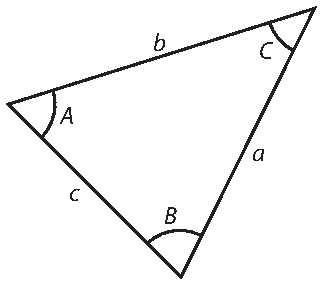
\includegraphics[width=0.4\textwidth]{triangle}
\caption{\label{fig:cosine} Guide for angles and distances when using the cosine rule.}
\end{figure}
%

\subsection{Optimisation}
This problem can be solved using simpler (and faster) code using NumPy arrays. Rewrite your code from the problam to use arrays and compare your results to your original version (you should get the same results). You might need to reconsider your algorithm to decide how to best use arrays to solve this problem.

\bibliographystyle{rsc}
\bibliography{handout_2}

\end{document}
